% geomdif_ej.tex 
% Fichero principal
%
% Copyright (C) 2025 José A. Navarro Ramón <janr.devel@gmail.com>
%
\documentclass[a4paper,10pt]{report}

% Paquetes
\usepackage{geomdif_ej.pkg}
% Definiciones
\usepackage{geomdif_ej.defs}

\begin{document}
% -----------------------------------------------------------------------------
% Añade 'Portadayy' al índice pdf.
\phantomsection \hypertarget{TOC}{}
\bookmark[level=0,dest=TOC]{Portada}
% Crea la portada.
\thispagestyle{empty}
% portada.tex
%
% Copyright (C) 2025 José A. Navarro Ramón <janr.devel@gmail.com>
%
% Portada del libro
\begin{tikzpicture}[remember picture, overlay]

% Coordenadas del punto central de la página a la altura donde irá la barra
\coordinate [below=6.5cm] (midpoint) at (current page.north);

% Barra superior
\node [name = colourbar,
anchor = base,
fill = orange!80!white,
text = black,
minimum width = \paperwidth,
minimum height = 1cm] at (midpoint)
{\hspace*{5cm}\LARGE{\textmd{\textsc{MATEMÁTICAS PARA LA FÍSICA}}}};
%{\hspace*{5cm}\LARGE{\textmd{\textsc{UNIVERSIDAD POLITÉCNICA DE CARTAGENA}}}};

% Set coordinate system origin
% Upper colour
\begin{scope}[shift=(colourbar.north west)]
\filldraw[fill=gray!15!white] (0,0) rectangle (current page.north east);
\end{scope}

% Set coordinate system origin
% Bottom colour
\begin{scope}[shift=(colourbar.south west)]
\filldraw[fill=white!20!white] (0,0) rectangle (current page.south east);
%\node[text=black]
%	at (15.6,-15) {\Huge\textbf{TEMAS 7, 8 y 9.}};
\end{scope}

% Define the point where the logo will go
\coordinate[right=4cm] (logo) at (colourbar.west);

% Set coordinate system origin
% The whole logo structure and the title image
\begin{scope}[shift=(logo)]
% Draw the two circles
\filldraw[circular drop shadow={shadow scale=1.003},
	fill=yellow!8,draw=black,thick]
	(0.0,0.00) circle (1.9cm);
\filldraw[fill=yellow!8,draw=black] (0.0,0.00) circle (1.48cm);

% IES
\path [postaction={decoration={text along path, text={CURSO DE},
	text align=fit to path}, decorate}]
	(140:1.55cm) arc (140:40:1.55cm);
% MARIANO
%\path [postaction={decoration={text along path, text={EJERCICIOS},
%	text align=fit to path}, decorate}]
%	(200:1.81cm) arc (200:265:1.81cm);
\path [postaction={decoration={text along path, text={F{Í}SICA},
	text align=fit to path}, decorate}]
	(190:1.81cm) arc (190:260:1.81cm);
% BAQUERO
\path [postaction={decoration={text along path, text={TE{Ó}RICA},
	text align=fit to path}, decorate}]
	(270:1.81cm) arc (270:350:1.81cm);
% Left star
\node[star,draw=black!70!white,fill=gray,
	minimum size=2mm,star point ratio=2.5,
	inner sep=0pt,rotate=-15] at (155:1.68cm) {};
% Right star
\node[star,draw=black!70!white,fill=gray,
	fill=black,minimum size=2mm,star point ratio=2.5,
	inner sep=0pt,rotate=15] at (25:1.68cm) {};
% Logo del IES Mariano Baquero
\node[yshift=0.6em] {
\includegraphics[width=2.5cm]
	{img/logo/cat2.png}};
%\node[yshift=0.6em] {\includegraphics[width=3.0cm]
%	{img/logo/logoiesmb-100x55}};

\node[yshift=-9.8cm,xshift=+6.4cm] {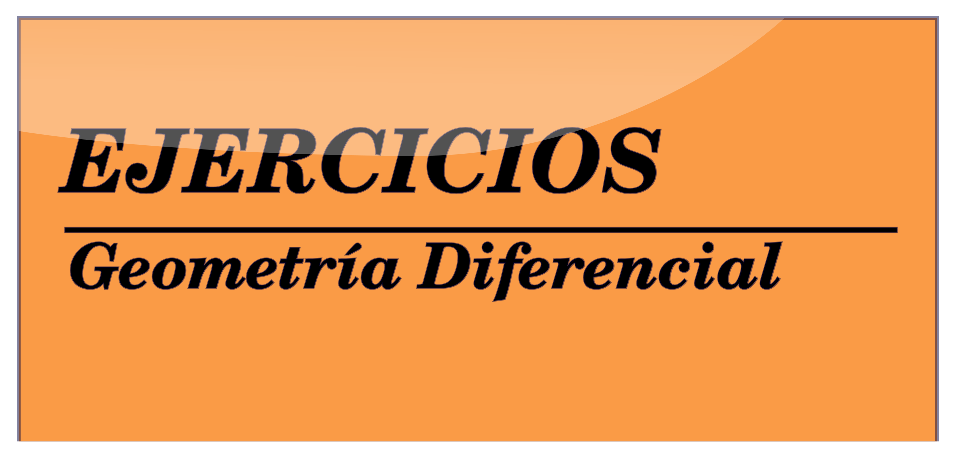
\includegraphics[width=17cm]
  {img/titulo/geomdif_ej-orange.eps}};

\node[yshift=-13.2cm,xshift=+11.9cm] {\large\fontPortada\sl\today --\currenttime};

\end{scope}


\end{tikzpicture}


%%% Local Variables:
%%% coding: utf-8
%%% mode: latex
%%% TeX-engine: luatex
%%% TeX-master: "../geomdif_ej.tex"
%%% End:

% -----------------------------------------------------------------------------
% -----------------------------------------------------------------------------
% Añade 'Contenidos' al índice pdf.
\hypertarget{Contents}{} \phantomsection
\bookmark[level=0,dest=Contents]{Contenidos}
% Estilo de página como 'empty' pero con número de página.
\pagestyle{plain}
% Crea la tabla de contenidos.
% tablacontenidos.tex
% Tabla de contenidos.
%
% Copyright (C) 2025 José A. Navarro Ramón <janr.devel@gmail.com>
%

\begin{tcolorbox}[breakable,enhanced jigsaw,title={Contenidos},fonttitle=\bfseries\Large,
  colback=yellow!10!white,colframe=red!50!black,before=\par\bigskip\noindent,
  interior style={fill overzoom image=goldshade.png,fill image opacity=0.25},
  colbacktitle=red!50!yellow!75!black,
  enlargepage flexible=\baselineskip,pad at break*=3mm,
  watermark color=yellow!75!red!25!white,
  watermark text={\bfseries\Large Contenidos},
  attach boxed title to top center={yshift=-0.25mm-\tcboxedtitleheight/2,yshifttext=2mm-\tcboxedtitleheight/2},
  boxed title style={enhanced,boxrule=0.5mm,
    frame code={ \path[tcb fill frame] ([xshift=-4mm]frame.west) -- (frame.north west)
    -- (frame.north east) -- ([xshift=4mm]frame.east)
    -- (frame.south east) -- (frame.south west) -- cycle; },
    interior code={ \path[tcb fill interior] ([xshift=-2mm]interior.west)
    -- (interior.north west) -- (interior.north east)
    -- ([xshift=2mm]interior.east) -- (interior.south east) -- (interior.south west)
    -- cycle;}  },
  drop fuzzy shadow]
\makeatletter
\@starttoc{toc}
\makeatother
\end{tcolorbox}


%%% Local Variables:
%%% coding: utf-8
%%% mode: latex
%%% TeX-engine: luatex
%%% TeX-master: "../geomdif_ej.tex"
%%% End:

% -----------------------------------------------------------------------------
% -----------------------------------------------------------------------------
%\part{Ejercicios}
%
\renewcommand*{\tipoDocumento}{ejercicios}
\renewcommand*{\parte}{EJERCICIOS DE GEOMETRÍA DIFERENCIAL}
% ------ Matemáticas -----------------------
\setcounter{isheet}{1}
\renewcommand*{\mainsubject}{Conceptos básicos de topología}
\phantomsection \addcontentsline{toc}{section}{\theisheet. \mainsubject}
\pagestyle{ejercicios}
% topologia.tex
%
% Copyright (C) 2025 José A. Navarro Ramón <janr.devel@gmail.com>
%
% ---------------------------------------------------------------------------
% ---------------------------------------------------------------------------
% HOJA
% ---------------------------------------------------------------------------
% ---------------------------------------------------------------------------
%\phantomsection
%\addcontentsline{toc}{subsection}{Hoja 1}
\setcounter{isubsheet}{1}

% Añade 'Contenidos' al índice pdf.
% \bookmark[level=2,dest=section]{Hoja 1}
% Nombre de enlace: 'cc1.2'
\pdfbookmark[2]{Hoja 1}{mathj01}

\begin{ejercicio}
% --------------------------------------------------------------------------
% Convergencia única de una sucesión de puntos en un espacio métrico
% --------------------------------------------------------------------------
\item
  Suponga una sucesión convergente de puntos en un espacio métrico.
  Demuestre que este límite es único.

% ...........................................................................
  \showSolved{res/topologia}{topologia-001.pdf}
% ...........................................................................
\medskip
{\color{gray}
\hrule
}

% --------------------------------------------------------------------------
% Stronger metrics than others
% --------------------------------------------------------------------------
\item
  Demuestre que si la métrica $d^{(2)}$ induce una topología más fuerte que la
  métrica $d^{(1)}$, entonces una sucesión $d^{(2)}$-convergente es
  automáticamente $d^{(1)}$-convergente.

% ...........................................................................
  \showSolved{res/topologia}{topologia-002.pdf}
% ...........................................................................
\medskip
{\color{gray}
\hrule
}


%% --------------------------------------------------------------------------
%%  Matrices de rotación
%% --------------------------------------------------------------------------
%\item
%  \begin{subejercicio}
%  \item Pruebe que la matriz de rotación $2\times 2$
%    \[
%      \begin{pNiceMatrix}
%        \overline{A}_y\\
%        \overline{A}_z
%      \end{pNiceMatrix}
%      =
%      \begin{pNiceMatrix}
%        \cos\phi & \sin\phi\\
%        -\sin\phi & \cos\phi
%      \end{pNiceMatrix}
%      \begin{pNiceMatrix}
%        A_y\\
%        A_z
%      \end{pNiceMatrix}
%    \]
%    preserva el producto escalar. Esto es, muestre que
%    \[
%    \overline{A}_y\,\, \overline{B}_y + \overline{A}_z\,\, \overline{B}_z
%    = A_y B_y + A_z B_z
%  \]
%\item ¿Qué restricciones deben cumplir los elementos $R_{ij}$ de la matriz
%  de rotación en tres dimensiones
%  \[
%    \begin{pNiceMatrix}
%      \overline{A}_x\\
%      \overline{A}_y\\
%      \overline{A}_z
%    \end{pNiceMatrix}
%    =
%    \begin{pNiceMatrix}
%      R_{xx} & R_{xy} & R_{xz}\\
%      R_{yx} & R_{yy} & R_{yz}\\
%      R_{zx} & R_{zy} & R_{zz}\\
%    \end{pNiceMatrix}
%    \begin{pNiceMatrix}
%      A_x\\
%      A_y\\
%      A_z
%    \end{pNiceMatrix}
%  \]
%  para que se conserve la longitud de $\vvv{A}$ (para todos los vectores $\vvv{A}$)?
%  \end{subejercicio}
%
%  % ...........................................................................
%  {\footnotesize \textcolor{gray}{[No resuelto]}}
%  %\showSolved{res/matematicas}{matematicas-008.pdf}
%% ...........................................................................
%%\medskip
%%{\color{gray}
%%\hrule
%%}
%
%% #########################################################################################
%% #########################################################################################
%% #########################################################################################
%
%\clearpage
%% \phantomsection
%%\addcontentsline{toc}{subsection}{Hoja 1}
%%\setcounter{isubsheet}{2}
%\stepcounter{isubsheet} 
%
%% Añade 'Contenidos' al índice pdf.
%% \bookmark[level=2,dest=section]{Hoja 1}
%% Nombre de enlace: 'cc1.2'
%\pdfbookmark[2]{Hoja 2}{mathj02}
%
%% --------------------------------------------------------------------------
%%  Matriz de rotación
%% --------------------------------------------------------------------------
%\item Encuentre la matriz de transformación $\mmm{R}$ que describa una rotación
%  de \ang{120} alrededor de un eje que pase por el origen y por el punto $(1,1,1)$.
%  La rotación debe ser antihoraria en cuando se observa el eje hacia el origen.
%
%  % ...........................................................................
%  {\footnotesize \textcolor{gray}{[No resuelto]}}
%  %\showSolved{res/matematicas}{matematicas-009.pdf}
%% ...........................................................................
%\medskip
%{\color{gray}
%\hrule
%}
%
%  
%  % --------------------------------------------------------------------------
%  % Gradiente
%  % --------------------------------------------------------------------------
%\item Suponga que $f$ es una función de dos variables, $y$ y $z$.
%  Demuestre que el gradiente
%  $\vvv{\nabla} f = (\partial f/\partial y)\xhat{y} + (\partial f/\partial z)\xhat{z}$
%  se transforma como un vector bajo rotaciones.
%  \[
%    \begin{pNiceMatrix}
%      \overline{A}_y\\
%      \overline{A}_z
%    \end{pNiceMatrix}
%    =
%    \begin{pNiceMatrix}
%      \cos\phi & \sin\phi\\
%      -\sin\phi & \cos\phi
%    \end{pNiceMatrix}
%    \begin{pNiceMatrix}
%      A_y\\
%      A_z
%    \end{pNiceMatrix}
%  \]
%  [Pista:
%  $(\partial f/\partial\overline{y})(\partial y/\partial\overline{y})
%  + (\partial f/\partial\overline{z}) (\partial z/\partial\overline{z})$,
%  y la fórmula análoga para $\partial f/\partial\overline{z}$. Sabemos que
%  $\overline{y} = y\cos\phi + z\sin\phi$ y $\overline{z} = -y\sin\phi + z\cos\phi$;
%  ``resuelva'' estas ecuaciones para $y$ y $z$ (como funciones de $\overline{y}$ y
%  $\overline{z}$), y calcule las derivadas intermedias $\partial y/\partial\overline{y}$,
%  $\partial z/\partial\overline{y}$, etc.]
%  
%  % ...........................................................................
%  {\footnotesize \textcolor{gray}{[No resuelto]}}
%  % \showSolved{res/matematicas}{matematicas-014.pdf}
%  % ...........................................................................
%  % \medskip
%  % {\color{gray}
%  % \hrule
%  % }
  
%  \medskip
%  {\color{gray}
%    \hrule
%  }
 
  
\end{ejercicio}


%%% Local Variables:
%%% coding: utf-8
%%% mode: latex
%%% TeX-engine: luatex
%%% TeX-master: "../geomdif_ej.tex"
%%% End:

% ------ Campos ----------------------------
%\renewcommand*{\mainsubject}{Electrostática}
%\addtocounter{isheet}{1}
%\phantomsection \addcontentsline{toc}{section}{\theisheet. \mainsubject}
%\include{./ejercicios/ed-electrostatica}

% -----------------------------------------------------------------------------
\end{document}

%%% Local Variables:
%%% coding: utf-8
%%% mode: latex
%%% TeX-engine: luatex
%%% TeX-master: t
%%% End:
